\documentclass[12pt]{ctexart}
\usepackage{geometry}
\geometry{a4paper, margin=1in}
\usepackage{amsmath}
\usepackage{graphicx}
\usepackage{multirow}
\usepackage{setspace}
\usepackage{caption}
\usepackage{float} % For [H] table placement
\usepackage{booktabs} % For professional looking tables
\usepackage{verbatim}
\usepackage{hyperref}
\usepackage{xcolor}
\usepackage{listings}
\usepackage{tabularx}
\usepackage{longtable}
\usepackage{array} % For custom column types
\usepackage{longtable} % For tables that span multiple pages
\usepackage{pythonhighlight}

% 格式设置
\setstretch{1.5}          % 1.5倍行距
\setlength{\parindent}{2em} % 首行缩进2字符

% 封面模板
\newcommand{\cover}[6]{
  \begin{center}
    {\LARGE \bfseries 《分布式能源系统概论》}\\[1em]
    {\Large \bfseries 实践作业}\\[2em] % Made "实践作业" bold
    
    \begin{tabular}{>{\raggedright}p{3cm}l} % Aligned labels to the left
      作业题目: & \underline{\makebox[8cm][s]{#1}} \\
      专~~~~业: & 能源与动力工程 \\
      班~~~~级: & 2023级能源与动力工程一班(化能杨班) \\
      学生姓名: & 唐玮嘉 \\
      学~~~~号: & 2023428020130 \\
      指导教师: & 陶实 副教授 \\
      年~月~日: & \underline{\makebox[4cm][s]{#2}} \\
    \end{tabular}
  \end{center}
  \vspace{2em}
}

\begin{document}

% 封面
\cover{分布式能源系统方案多属性综合评价研究}{\today}

% 课程论文任务书
\newpage
\section*{课程论文任务书}
专业:能源与动力工程 \quad 班级:2023级能源与动力工程一班(化能杨班)

\begin{tabularx}{\textwidth}{|>{\raggedright\arraybackslash}p{3cm}|X|} % Simplified to two columns
  \hline
  学生姓名 & 唐玮嘉 \\
  \hline
  学号 & 2023428020130 \\
  \hline
  论文题目 & \underline{分布式能源系统方案多属性综合评价研究} \\
  \hline
  \multirow{3}{=}{\centering\arraybackslash 设计目的、主要内容及要求} 
    & 
      \textbf{设计目的:} \par
      本次实践旨在通过对给定的五个分布式能源系统方案进行多属性综合评价,深化对分布式能源系统复杂性的理解。核心目的是应用层次分析法(AHP)和灰色关联分析(GRA)相结合的决策方法,科学、客观地评估各方案的优劣,并筛选出相对最优方案。同时,培养运用编程工具(Python)处理数据、实现评价模型及分析结果的能力。
      \par \vspace{0.5em}
      \textbf{主要内容:} \par
      1. 数据准备与指标体系构建:整理原始数据,明确经济性、环境性、社会性、性能及噪声五个准则层及其下属的12个基层评价指标,并区分指标的正逆属性。 \par
      2. 指标预处理:对定性评级指标(技术先进性、安全性、维护方便性)采用模糊隶属函数进行量化;对定量指标进行无量纲化处理,统一为“越高越优”型。 \par
      3. 权重计算:基于提供的判断矩阵,运用AHP法计算准则层权重和各准则层下指标的局部权重,进而得到各基层指标的全局权重,并进行一致性检验(CR)。 \par
      4. 综合评价:构建理想参考序列,计算各方案的灰色关联系数,并结合全局权重计算各方案的灰色加权关联度,据此对方案进行排序。 \par
      5. 结果分析与讨论:展示各阶段计算结果,分析最优方案的特性,并对评价过程中(如AHP判断矩阵一致性)的问题进行反思。
      \par \vspace{0.5em}
      \textbf{要求:} \par
      1. 评价过程科学严谨,方法运用得当。 \par
      2. 数据处理准确,计算结果可靠。 \par
      3. 论文结构清晰,论述充分,图表规范。 \par
      4. 对评价方法和结果有独立的思考和见解。
  \\
  \hline
  进度安排 & \multicolumn{1}{p{\dimexpr\textwidth-4cm-4\tabcolsep}|}{% 
    (本次报告侧重于方法实现与结果分析,具体进度从略)
  } \\
  \hline
  主要参考资料 & \multicolumn{1}{p{\dimexpr\textwidth-4cm-4\tabcolsep}|}{%
    \begin{enumerate}
        \item 课程提供的“附件1:冷热电联供系统综合评价”相关章节。
        \item 课程提供的“附件2:定性指标定量化及指标权重计算”相关说明。
        \item 课程提供的原始数据表 (`order-63.txt`)。
        \item (未额外参考外部文献)
    \end{enumerate}
  } \\
  \hline
  指导教师签字 & \underline{\makebox[\dimexpr\textwidth-4cm-5\tabcolsep][s]{}} \\
  \hline
\end{tabularx}

\newpage
% 摘要与关键词
\section*{摘 要}
\noindent 分布式能源系统因其高效、灵活等优点受到广泛关注,但其方案选择涉及经济、环境、社会、性能等多重属性,是一个复杂的多目标决策问题。本文针对给定的五个分布式能源系统备选方案,采用层次分析法(AHP)与灰色关联分析(GRA)相结合的综合评价方法。首先,构建了包含经济性、环境性、社会性、性能和噪声五个准则层及12个基层指标的评价体系。对原始数据进行预处理:定性指标通过模糊隶属函数量化,定量指标进行无量纲化处理,均转化为“越高越优”型。其次,利用AHP法确定了各指标的全局权重,并对判断矩阵进行了一致性检验。最后,通过GRA计算各方案与理想方案的灰色加权关联度,并据此进行排序。评价结果表明,方案D的综合灰色关联度最高(0.8608),为相对最优方案。本文详细阐述了评价模型的构建、数据处理流程、权重计算及综合评价过程,并对AHP判断矩阵的一致性问题进行了讨论,为分布式能源系统的方案优选提供了一种系统化的分析思路和方法借鉴。

\vspace{1em}
\noindent \textbf{关键词:} 分布式能源系统;综合评价;层次分析法 (AHP);灰色关联分析 (GRA);模糊量化;方案优选

\newpage
% 目录
\tableofcontents
\addcontentsline{toc}{section}{目 录} % 添加目录到目录页

\newpage
% 正文
\section{引言}
分布式能源系统作为一种新型的能源供应方式,具有能源利用效率高、环境影响小、供能可靠性强等潜在优势,在现代能源体系转型中扮演着日益重要的角色。然而,分布式能源项目的方案设计与选择往往面临多方面的权衡,涉及经济投入与回报、环境排放、社会接纳度、系统运行性能等多个维度的考量。这些属性之间可能存在冲突和不可公度性,使得方案比选成为一个典型的多属性决策难题。

为了对不同的分布式能源系统方案进行科学、合理的评估和优选,需要建立一套系统性的综合评价方法。单一维度的评价(如仅考虑经济性)往往难以全面反映方案的综合优劣。层次分析法 (AHP) 是一种成熟的将定性判断与定量分析相结合的决策方法,善于处理复杂系统中的权重确定问题。灰色关联分析 (GRA) 则是一种基于数据序列几何相似性的分析方法,适用于样本量较小、信息不完全情况下的系统分析和方案排序。

本次实践作业旨在针对给定的五个分布式能源系统方案(分别标记为方案A、B、C、D、E),运用AHP与GRA相结合的方法进行综合评价。通过构建合理的评价指标体系,对原始数据进行科学的预处理,确定各评价指标的相对重要性(权重),并最终计算各方案的综合评价值,以期筛选出相对最优的系统方案,并在此过程中加深对多属性决策方法在能源系统评价中应用的理解。

\section{评价方法与模型}
本研究采用的综合评价流程主要包括:构建评价指标体系、数据预处理(定性指标模糊量化与定量指标无量纲化)、基于AHP的指标权重计算以及基于GRA的方案综合评价与排序。

\subsection{评价指标体系}
根据分布式能源系统综合评价的常见维度,结合所提供的数据,构建了包含5个准则层和12个基层指标的评价体系,如表\ref{tab:indicators}所示。

\begin{table}[H]
  \centering
  \caption{分布式能源系统综合评价指标体系}
  \label{tab:indicators}
  \begin{tabular}{lll}
    \toprule
    准则层 (Level 1) & 基层指标 (Level 2) & 原始指标性质 \\
    \midrule
    \multirow{4}{*}{经济性 (F1)} 
        & 初投资 (元) & 逆指标 (\(\downarrow\)) \\
        & 投资回收期 (年) & 逆指标 (\(\downarrow\)) \\
        & 总费用年值 (元) & 逆指标 (\(\downarrow\)) \\
        & 净现值 (元) & 正指标 (\(\uparrow\)) \\
    \midrule
    \multirow{3}{*}{环境性 (F2)} 
        & 氮氧化物 (g/kW·h) & 逆指标 (\(\downarrow\)) \\
        & CO (g/kW·h) & 逆指标 (\(\downarrow\)) \\
        & CO₂ (g/kW·h) & 逆指标 (\(\downarrow\)) \\
    \midrule
    \multirow{3}{*}{社会性 (F3)} 
        & 技术先进性 (评级1-5) & 正指标 (\(\uparrow\)) \\
        & 安全性 (评级1-5) & 正指标 (\(\uparrow\)) \\
        & 维护方便性 (评级1-5) & 正指标 (\(\uparrow\)) \\
    \midrule
    性能 (F4) & 一次能源比 & 逆指标 (\(\downarrow\)) \\
    \midrule
    噪声 (F5) & 噪声 (dB) & 逆指标 (\(\downarrow\)) \\
    \bottomrule
  \end{tabular}
\end{table}
注:评级1-5中,5为最优。一次能源比实为一次能源利用率的倒数或相关概念,此处按逆指标处理。

\subsection{数据预处理}
为消除不同指标量纲和正逆属性的差异,需对原始数据进行预处理。

\subsubsection{定性指标模糊量化}
对于技术先进性、安全性、维护方便性这三个定性指标(原始数据为1-5的评级,5为最优),采用课程附件中提供的模糊隶属函数进行量化。该函数将离散的评级映射到[0,1]区间内的连续值,评级越高,量化值越大。其表达式为:
\[
f(x) = 
\begin{cases} 
[1 + \alpha(x-\beta)^{-2}]^{-1} & 1 \le x \le 3 \\
a \ln x + b & 3 < x \le 5 
\end{cases}
\]
其中,常数 \(\alpha=1.1086, \beta=0.8942, a=0.3915, b=0.3699\)。根据此函数,评级1, 2, 3, 4, 5分别近似量化为0.01, 0.5245, 0.8, 0.9126, 1.0。

\subsubsection{定量指标无量纲化}
对定量指标,采用极差变换法进行无量纲化处理,使其值也落入[0,1]区间。
对于正指标(效益型,越大越优,如净现值),其标准化公式为:
\[ z_{ij} = \frac{x_{ij} - \min(x_j)}{\max(x_j) - \min(x_j)} \]
对于逆指标(成本型,越小越优,如初投资),其标准化公式为:
\[ z_{ij} = \frac{\max(x_j) - x_{ij}}{\max(x_j) - \min(x_j)} \]
其中 \(x_{ij}\) 为第 \(i\) 个方案在第 \(j\) 个指标上的原始值,\(\min(x_j)\) 和 \(\max(x_j)\) 分别为所有方案在第 \(j\) 个指标上的最小值和最大值。若某指标在所有方案中取值相同,则其标准化值均取1.0。
经过预处理后,所有指标均转化为“越高越优”型。

\subsection{层次分析法 (AHP) 确定权重}
AHP通过构建判断矩阵来量化各元素间的相对重要性,然后计算矩阵的最大特征值及其对应的特征向量,该归一化特征向量即为各元素的权重。为检验判断矩阵的逻辑一致性,引入一致性比例CR:
\[ CR = \frac{CI}{RI} = \frac{(\lambda_{\max} - n)}{(n-1)RI} \]
其中 \(\lambda_{\max}\) 为判断矩阵的最大特征值,\(n\) 为矩阵阶数,RI为平均随机一致性指标。通常认为当 \(CR < 0.1\) 时,判断矩阵具有满意的一致性。

本研究中,权重计算分两层:
\begin{enumerate}
    \item \textbf{准则层权重 (Level 1)}:构建经济性(F1)、环境性(F2)、社会性(F3)、性能(F4)、噪声(F5)五个准则的5x5判断矩阵,计算其权重 \(W_L1 = (w_{F1}, w_{F2}, w_{F3}, w_{F4}, w_{F5})\)。
    \item \textbf{指标层相对权重 (Level 2)}:分别对经济性(4个子指标)、环境性(3个子指标)、社会性(3个子指标)构建其内部子指标的判断矩阵,计算其局部权重。性能和噪声层面各仅含一个指标,其局部权重为1。
    \item \textbf{全局权重}:基层指标的全局权重由其所属准则的权重与该指标在准则内的局部权重相乘得到,并进行归一化。
\end{enumerate}
所使用的判断矩阵主要参考已有代码中的设定。

\subsection{灰色关联分析 (GRA)}
GRA通过计算比较序列(各方案的指标序列)与参考序列(理想方案的指标序列)之间的几何相似程度来衡量它们的关联性。对于已全部转化为“越高越优”型的标准化数据,理想参考序列可设为各项指标值均为1的序列 \(Z_0 = (z_{01}, z_{02}, \dots, z_{0m})\),其中 \(z_{0j}=1\)。
第 \(i\) 个方案的第 \(j\) 个指标 \(z_{ij}\) 与理想指标 \(z_{0j}\) 的灰色关联系数 \(\xi_{ij}\) 计算公式为:
\[ \xi_{ij} = \frac{\min_i \min_j |z_{0j} - z_{ij}| + \rho \cdot \max_i \max_j |z_{0j} - z_{ij}|}{|z_{0j} - z_{ij}| + \rho \cdot \max_i \max_j |z_{0j} - z_{ij}|} \]
其中 \(\rho \in [0,1]\) 为分辨系数,通常取0.5。
第 \(i\) 个方案的加权灰色关联度 \(R_i\) 由其各指标的关联系数与对应的全局权重 \(w_j\) 加权求和得到:
\[ R_i = \sum_{j=1}^{m} w_j \xi_{ij} \]
关联度 \(R_i\) 越大,表示方案 \(i\) 越接近理想方案,即综合评价越优。

\section{评价结果与分析}
\subsection{指标预处理结果}
对原始数据进行模糊量化和无量纲化处理后,得到的各方案在12个基层指标上的评价值(均已转化为越高越优型)如表\ref{tab:processed_data}所示。

\begin{table}[H]
  \centering
  \caption{预处理后的指标评价值 (越高越优)}
  \label{tab:processed_data}
  \resizebox{\textwidth}{!}{%
  \begin{tabular}{lrrrrrrrrrrrr}
    \toprule
    方案 & 初投资 & 回收期 & 总费用 & 净现值 & NOx & CO & CO₂ & 先进性 & 安全性 & 维护性 & 能耗比 & 噪声 \\
    \midrule
    方案A & 0.7500 & 0.7500 & 0.7500 & 0.2500 & 0.7500 & 1.0000 & 0.5000 & 1.0000 & 0.0100 & 0.8000 & 0.0000 & 1.0000 \\
    方案B & 0.2500 & 1.0000 & 0.0000 & 0.7500 & 0.5000 & 0.0000 & 0.0000 & 0.8000 & 1.0000 & 0.0100 & 0.7500 & 0.2500 \\
    方案C & 0.0000 & 0.2500 & 0.5000 & 0.5000 & 0.2500 & 0.5000 & 0.2500 & 0.5245 & 0.5245 & 0.9126 & 0.2500 & 0.5000 \\
    方案D & 1.0000 & 0.5000 & 0.2500 & 1.0000 & 0.0000 & 0.7500 & 1.0000 & 0.0100 & 0.8000 & 1.0000 & 1.0000 & 0.7500 \\
    方案E & 0.5000 & 0.0000 & 1.0000 & 0.0000 & 1.0000 & 0.2500 & 0.7500 & 0.9126 & 0.9126 & 0.5245 & 0.5000 & 0.0000 \\
    \bottomrule
  \end{tabular}%
  }
\end{table}
注:表中数值为四舍五入到小数点后4位的结果。先进性、安全性、维护性为模糊量化结果,其余为无量纲化结果。

\subsection{权重计算结果}
\subsubsection{准则层 (Level 1) 权重}
经济性(F1)、环境性(F2)、社会性(F3)、性能(F4)和噪声(F5)五个准则的判断矩阵及计算得到的权重和一致性比例如表\ref{tab:level1_weights}所示。
\begin{table}[H]
  \centering
  \caption{准则层权重及一致性检验}
  \label{tab:level1_weights}
  \begin{tabular}{lcccccr}
    \toprule
    准则 & F1 & F2 & F3 & F4 & F5 & 权重 \\
    \midrule
    F1 (经济) & 1 & 5 & 9 & 3 & 7 & 0.4728 \\
    F2 (环境) & 1/5 & 1 & 6 & 1/3 & 1/4 & 0.0834 \\
    F3 (社会) & 1/9 & 1/6 & 1 & 1/5 & 1/3 & 0.0325 \\
    F4 (性能) & 1/3 & 3 & 5 & 1 & 9 & 0.3049 \\
    F5 (噪声) & 1/7 & 4 & 3 & 1/9 & 1 & 0.1063 \\
    \midrule
    \multicolumn{6}{r}{\(\lambda_{\max} = 6.0094\)} & \(CR = 0.2273\) \\
    \bottomrule
  \end{tabular}
\end{table}
准则层判断矩阵的 \(CR = 0.2273\),大于0.1,表明该判断矩阵的一致性较差。这意味着赋予准则层各因素相对重要性的判断可能存在一定的逻辑矛盾。在实际决策中,需要对该判断矩阵进行调整以提高一致性。本次实践仍基于此结果进行后续计算,但需注意此局限性对最终结果可能产生的影响。

\subsubsection{指标层局部权重与全局权重}
各准则层下属指标的局部权重通过AHP法计算,其中环境性指标 (\(CR=0.0516\)) 和社会性指标 (\(CR=0.0624\)) 的判断矩阵一致性良好。然而,经济性指标的判断矩阵一致性同样较差 (\(CR=0.3283\))。性能和噪声层面各仅有一个指标,局部权重为1。各基层指标的全局权重由准则层权重与相应的局部权重乘积并归一化得到,结果如表\ref{tab:global_weights}所示。

\begin{table}[H]
  \centering
  \caption{基层指标全局权重}
  \label{tab:global_weights}
  \begin{tabular}{lr|lr}
    \toprule
    指标 & 全局权重 & 指标 & 全局权重 \\
    \midrule
    初投资 & 0.2737 & CO₂ & 0.0182 \\
    投资回收期 & 0.0704 & 技术先进性 & 0.0091 \\
    总费用年值 & 0.0260 & 安全性 & 0.0211 \\
    净现值 & 0.1028 & 维护方便性 & 0.0023 \\
    氮氧化物 & 0.0576 & 一次能源比 & 0.3049 \\
    CO & 0.0076 & 噪声 & 0.1063 \\
    \bottomrule
    \multicolumn{4}{r}{注:权重之和为1.0000} \\
  \end{tabular}
\end{table}
从全局权重看,“一次能源比”(性能层面)和“初投资”(经济性层面)是最重要的两个指标,其次是“噪声”和“净现值”。社会性层面的指标以及环境性中的CO指标权重相对较低。

\subsection{灰色关联分析结果}
\subsubsection{灰色关联系数矩阵}
各方案的各预处理指标与理想值(全1序列)的灰色关联系数 (\(\xi_{ij}\),取\(\rho=0.5\))如表\ref{tab:gra_coeffs}所示。关联系数值越大,表明该方案在该项指标上越接近理想状态。

\begin{table}[H]
  \centering
  \caption{灰色关 联系数矩阵 (\(\xi_{ij}\))}
  \label{tab:gra_coeffs}
  \resizebox{\textwidth}{!}{%
  \begin{tabular}{lrrrrrrrrrrrr}
    \toprule
    方案 & 初投资 & 回收期 & 总费用 & 净现值 & NOx & CO & CO₂ & 先进性 & 安全性 & 维护性 & 能耗比 & 噪声 \\
    \midrule
    方案A & 0.6667 & 0.6667 & 0.6667 & 0.4000 & 0.6667 & 1.0000 & 0.5000 & 1.0000 & 0.3356 & 0.7143 & 0.3333 & 1.0000 \\
    方案B & 0.4000 & 1.0000 & 0.3333 & 0.6667 & 0.5000 & 0.3333 & 0.3333 & 0.7143 & 1.0000 & 0.3356 & 0.6667 & 0.4000 \\
    方案C & 0.3333 & 0.4000 & 0.5000 & 0.5000 & 0.4000 & 0.5000 & 0.4000 & 0.5126 & 0.5126 & 0.8513 & 0.4000 & 0.5000 \\
    方案D & 1.0000 & 0.5000 & 0.4000 & 1.0000 & 0.3333 & 0.6667 & 1.0000 & 0.3356 & 0.7143 & 1.0000 & 1.0000 & 0.6667 \\
    方案E & 0.5000 & 0.3333 & 1.0000 & 0.3333 & 1.0000 & 0.4000 & 0.6667 & 0.8513 & 0.8513 & 0.5126 & 0.5000 & 0.3333 \\
    \bottomrule
  \end{tabular}%
  }
\end{table}

\subsubsection{综合评价结果与排序}
将灰色关联系数与对应的全局指标权重加权求和,得到各方案的综合灰色加权关联度 \(R_i\),并进行排序,结果如表\ref{tab:final_ranking}所示。

\begin{table}[H]
  \centering
  \caption{各方案综合灰色关联度及排序}
  \label{tab:final_ranking}
  \begin{tabular}{crr}
    \toprule
    方案 & 综合灰色关联度 (\(R_i\)) & 排序 \\
    \midrule
    方案D & 0.8608 & 1 \\
    方案A & 0.5687 & 2 \\
    方案B & 0.5686 & 3 \\
    方案E & 0.5081 & 4 \\
    方案C & 0.4105 & 5 \\
    \bottomrule
  \end{tabular}
\end{table}
根据综合评价结果,方案D的综合灰色关联度最高(0.8608),为本次评价中的最优方案。方案A和方案B的关联度相近,分别位列第二和第三。方案E和方案C相对较差。
% 插入图片
\begin{figure}[H]
  \centering
  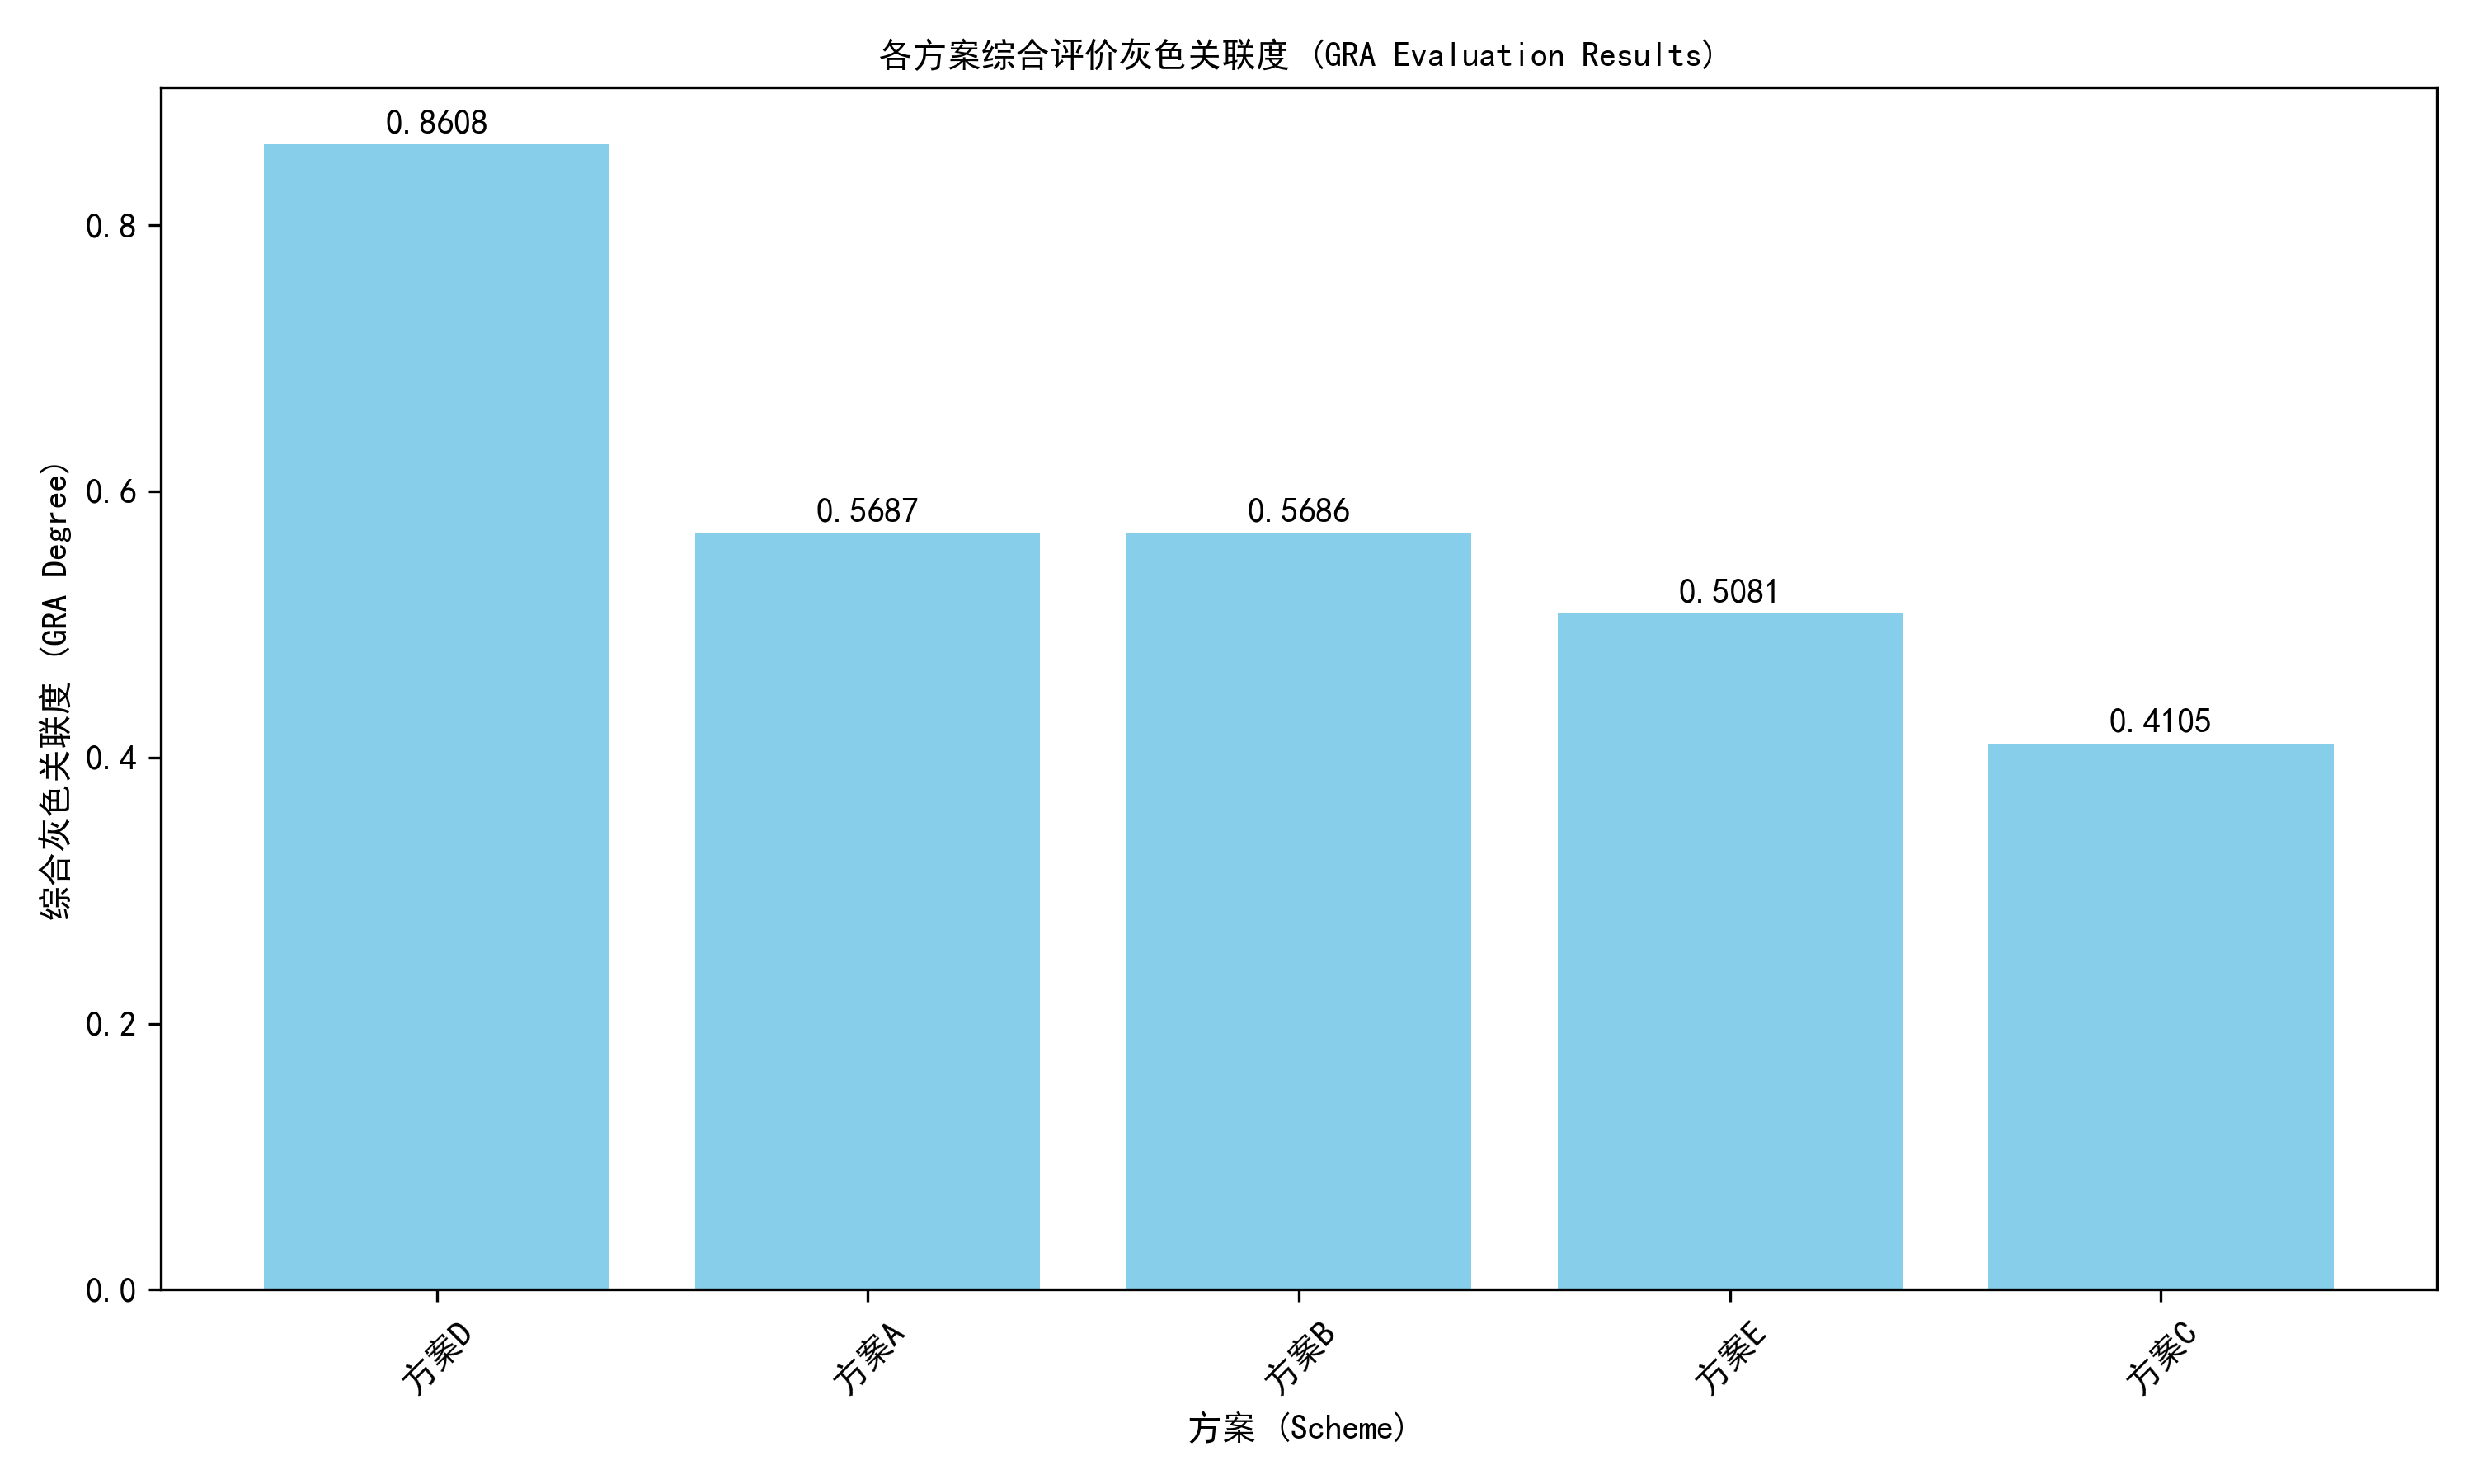
\includegraphics[width=0.8\textwidth]{../fig_综合评价结果_v2/GRA_Results_Comparison.png}
  \caption{灰色关联度排序图}
  \label{fig:gra_ranking}
\end{figure}

\subsection{结果讨论}
方案D之所以表现最优,从其预处理数据(表\ref{tab:processed_data})和关联系数(表\ref{tab:gra_coeffs})可以看出,它在多个权重较高的指标上表现突出或接近理想值:
\begin{itemize}
    \item \textbf{一次能源比} (全局权重0.3049): 方案D的预处理值为1.00 (最优),关联系数也为1.0000。
    \item \textbf{初投资} (全局权重0.2737): 方案D的预处理值为1.00 (最优),关联系数也为1.0000。
    \item \textbf{净现值} (全局权重0.1028): 方案D的预处理值为1.00 (最优),关联系数也为1.0000。
    \item \textbf{噪声} (全局权重0.1063): 方案D的预处理值为0.75,关联系数为0.6667,表现较好。
    \item \textbf{CO₂排放} (全局权重0.0182): 方案D的预处理值为1.00 (最优),关联系数也为1.0000。
\end{itemize}
尽管方案D在氮氧化物排放(预处理值0.00,关联系数0.3333)和技术先进性(预处理值0.01,关联系数0.3356)上表现不佳,但由于其在多个高权重指标上的显著优势,综合得分最高。

值得注意的是,本次评价中准则层和经济性指标层的AHP判断矩阵一致性较差 (CR > 0.1)。这意味着权重分配的可靠性受到一定影响。如果采用一致性更好的判断矩阵,各指标的全局权重可能会发生变化,从而可能影响最终的方案排序。在实际决策应用中,务必需要调整判断矩阵,确保其通过一致性检验,以获得更可信的评价结果。

\section{结论与思考}
本文运用层次分析法 (AHP) 和灰色关联分析 (GRA) 相结合的方法,对五个分布式能源系统方案进行了多属性综合评价。研究主要结论如下:
\begin{enumerate}
    \item 通过构建包含经济、环境、社会、性能和噪声五个方面的12个具体指标的评价体系,并对原始数据进行模糊量化和无量纲化处理,实现了不同性质指标的统一比较基础。
    \item 采用AHP法计算了各指标的全局权重,结果显示“一次能源比”、“初投资”、“噪声”和“净现值”是影响方案优选的关键因素。但需关注的是,部分判断矩阵的一致性检验未通过,提示权重结果的潜在不确定性。
    \item 基于GRA的综合评价结果表明,方案D以0.8608的最高综合关联度成为相对最优方案,主要得益于其在多个高权重指标上的优异表现。方案A、B、E、C依次排序。
\end{enumerate}

通过本次实践,可以深刻体会到多属性决策方法在复杂系统评价中的应用价值。AHP能够较好地处理权重确定的问题,将决策者的经验和判断融入模型;GRA则能在信息不完全的情况下,有效地对方案进行区分和排序。然而,AHP判断矩阵的构造和一致性调整是确保评价结果可靠性的关键环节,需要决策者投入足够的精力进行严谨的思考和判断。

对于分布式能源系统的评价而言,选择合适的评价指标并科学地确定其权重至关重要。未来的研究可以考虑引入更多利益相关者的偏好,或采用其他权重确定方法(如熵权法)与AHP进行对比,以期获得更为全面和鲁棒的评价结论。同时,针对AHP判断矩阵一致性差的问题,应深入分析原因并进行修正,这是提升决策科学性的必要步骤。本次作业虽存在此局限,但完整地展示了AHP-GRA方法的实施流程,为类似评价问题提供了有益的思路。

\section{附录}
\begin{python}
import os
import numpy as np
import pandas as pd
import matplotlib.pyplot as plt
from matplotlib.font_manager import FontProperties
import math

# --- Configuration & Constants ---
DATA_FILE = 'order-63.txt'
OUTPUT_DIR = 'fig_综合评价结果_v2' # Changed output directory
RHO_GRA = 0.5

ALPHA_FUZZY = 1.1086
BETA_FUZZY = 0.8942
A_FUZZY = 0.3915
B_FUZZY = 0.3699

# Matplotlib setup
if not os.path.exists(OUTPUT_DIR):
    os.makedirs(OUTPUT_DIR)
try:
    plt.rcParams['font.sans-serif'] = ['SimHei']
    plt.rcParams['axes.unicode_minus'] = False
    font = FontProperties(family='SimHei')
except:
    print("SimHei font not found, using default font for plots.")
    font = FontProperties()

# --- Helper Functions ---

def fuzzy_membership_function(x_qualitative):
    """
    Quantifies qualitative indicators using the fuzzy membership function.
    Input x_qualitative is a rating (1 to 5).
    f(1)=0.01, f(3)=0.8, f(5)=1.0
    Formula from PDF page 11:
    - [1 + alpha * (x - beta)^(-2)]^(-1)  for 1 <= x <= 3
    - a * ln(x) + b                       for 3 < x <= 5
    """
    x = float(x_qualitative) # Ensure float for calculations

    if not (1.0 <= x <= 5.0):
        # This should catch any out-of-range raw inputs if they occur
        raise ValueError(f"Qualitative input x={x} is out of the expected range [1, 5]")

    value = np.nan # Initialize to NaN to catch unhandled cases

    if 1.0 <= x <= 3.0: # This correctly includes x=1, x=2, and x=3
        # Term (x - BETA_FUZZY)^2
        # For x=1: (1 - 0.8942)^2 = (0.1058)^2 = 0.01119364
        # For x=2: (2 - 0.8942)^2 = (1.1058)^2 = 1.22279364
        # For x=3: (3 - 0.8942)^2 = (2.1058)^2 = 4.43438564
        # None of these are zero.
        denominator_of_power_term = (x - BETA_FUZZY)**2
        
        if abs(denominator_of_power_term) < 1e-12:
            # This case should not be hit with integer x in [1,3] and BETA_FUZZY=0.8942
            # If it were, it implies x is almost exactly BETA_FUZZY.
            # alpha / (small_number) -> large number
            # 1 / (1 + large_number) -> approaches 0
            print(f"Warning: (x - BETA_FUZZY)^2 is near zero for x={x}. Result may be imprecise.")
            value = 0.0 
        else:
            # Formula: 1.0 / (1.0 + ALPHA_FUZZY * (x - BETA_FUZZY)^(-2.0))
            # which is 1.0 / (1.0 + ALPHA_FUZZY / denominator_of_power_term)
            value = 1.0 / (1.0 + ALPHA_FUZZY / denominator_of_power_term)
            
    elif 3.0 < x <= 5.0: # This correctly includes x=4 and x=5
        # For x=4: 0.3915 * ln(4) + 0.3699 = 0.3915 * 1.38629 + 0.3699 = 0.54276 + 0.3699 = 0.91266
        # For x=5: 0.3915 * ln(5) + 0.3699 = 0.3915 * 1.60943 + 0.3699 = 0.63010 + 0.3699 = 1.00000
        value = A_FUZZY * math.log(x) + B_FUZZY
    
    if np.isnan(value):
        # This means x was in [1,5] but didn't match either if/elif block.
        # This should not happen if the conditions are 1<=x<=3 and 3<x<=5
        print(f"Error: No fuzzy value computed for x={x}. Check conditional logic.")
        
    return value

def calculate_ahp_weights(judgement_matrix):
    n = judgement_matrix.shape[0]
    if n == 0: return np.array([]), 0.0, 0.0
    if n == 1: return np.array([1.0]), 0.0, 1.0 # Single criterion

    eigenvalues, eigenvectors = np.linalg.eig(judgement_matrix)
    max_eigenvalue_index = np.argmax(eigenvalues.real)
    lambda_max = eigenvalues[max_eigenvalue_index].real
    w = eigenvectors[:, max_eigenvalue_index].real
    weights = w / np.sum(w)
    
    ci = (lambda_max - n) / (n - 1) if n > 1 else 0
    ri_values = {1:0, 2:0, 3:0.52, 4:0.89, 5:1.11, 6:1.25, 7:1.35, 8:1.40, 9:1.45, 10:1.49, 11:1.51, 12:1.52} # Updated RI from common sources
    ri = ri_values.get(n, 1.52) 
    if n > len(ri_values) and ri == ri_values[max(ri_values.keys())] : # Using RI for largest n if not found
         print(f"Warning: RI for n={n} not explicitly defined in lookup, using RI for n={max(ri_values.keys())}. CR accuracy may be affected.")

    cr = ci / ri if ri != 0 else (0 if ci == 0 else float('inf')) # Handle RI=0 for n=1,2
    return weights, cr, lambda_max

def normalize_quantitative_data(data_subset, indicator_types_subset):
    norm_data = np.zeros_like(data_subset, dtype=float)
    for j in range(data_subset.shape[1]):
        col_data = data_subset[:, j]
        min_val = np.min(col_data)
        max_val = np.max(col_data)
        
        if abs(max_val - min_val) < 1e-9: # Handles float comparison for equality
            # All values in the column are (practically) the same.
            # Normalized value should be 1.0 if the identical value is optimal,
            # or some mid-value (0.5) if it's neutral.
            # Given GRA expects higher is better, and if all are same, they are equally good/bad relative to each other.
            # If it's a positive indicator and all values are say 5, then (5-5)/(5-5) is problem.
            # Let's assign 1.0, implying they are all at the same (potentially optimal or non-differentiable) level.
            norm_data[:, j] = 1.0 
        elif indicator_types_subset[j] == 1:
            norm_data[:, j] = (col_data - min_val) / (max_val - min_val)
        else:
            norm_data[:, j] = (max_val - col_data) / (max_val - min_val)
    return norm_data

def grey_relational_analysis(processed_data, global_weights, rho=0.5):
    num_schemes, num_indicators = processed_data.shape
    if np.isnan(processed_data).any():
        print("Error: NaN values detected in data provided to GRA.")
        # You might want to return NaN arrays or raise an error
        nan_gra_coeffs = np.full((num_schemes, num_indicators), np.nan)
        nan_gra_degrees = np.full(num_schemes, np.nan)
        return nan_gra_coeffs, nan_gra_degrees

    reference_sequence = np.ones(num_indicators)
    abs_diff = np.abs(processed_data - reference_sequence)
    min_abs_diff_all = np.min(abs_diff)
    max_abs_diff_all = np.max(abs_diff)

    if abs(max_abs_diff_all) < 1e-9: # All processed data is identical to reference (all 1s)
        ksi = np.ones_like(processed_data)
    else:
        ksi = (min_abs_diff_all + rho * max_abs_diff_all) / (abs_diff + rho * max_abs_diff_all)
    
    if global_weights.ndim > 1: global_weights = global_weights.flatten()
    if len(global_weights) != num_indicators:
        raise ValueError(f"Weight/indicator mismatch for GRA: {len(global_weights)} vs {num_indicators}")
    gra_degree = np.dot(ksi, global_weights)
    return ksi, gra_degree

# --- Main Processing ---
def main():
    print("--- Comprehensive Evaluation of Distributed Energy Systems (v2) ---")

    raw_indicator_data_transposed = np.loadtxt(DATA_FILE, dtype=float)
    raw_indicator_data = raw_indicator_data_transposed.T
    scheme_names = [f'方案{chr(65+i)}' for i in range(raw_indicator_data.shape[0])]
    
    base_indicator_names = [
        '初投资', '投资回收期', '总费用年值', '净现值',
        '氮氧化物', 'CO', 'CO₂',
        '技术先进性', '安全性', '维护方便性',
        '一次能源比', '噪声'
    ]
    base_indicator_types = [0,0,0,1, 0,0,0, 1,1,1, 0,0] # Original nature
    qualitative_indicator_indices = [7, 8, 9]

    print(f"\nLoaded raw data for {raw_indicator_data.shape[0]} schemes x {raw_indicator_data.shape[1]} indicators.")
    df_raw_data = pd.DataFrame(raw_indicator_data, index=scheme_names, columns=base_indicator_names)
    print("Raw Data:")
    print(df_raw_data)

    # --- Indicator Preprocessing ---
    processed_data = np.zeros_like(raw_indicator_data, dtype=float)
    quantitative_indices = [i for i in range(len(base_indicator_names)) if i not in qualitative_indicator_indices]
    
    print("\n--- Fuzzifying Qualitative Indicators ---")
    for idx_qual in qualitative_indicator_indices:
        indicator_name_qual = base_indicator_names[idx_qual]
        # print(f"Processing Qualitative Indicator: {indicator_name_qual} (index {idx_qual})")
        for i_scheme in range(raw_indicator_data.shape[0]):
            scheme_name_qual = scheme_names[i_scheme]
            raw_value = raw_indicator_data[i_scheme, idx_qual]
            fuzzified_value = fuzzy_membership_function(raw_value)
            # print(f"  Scheme: {scheme_name_qual}, Raw: {raw_value}, Fuzzified: {fuzzified_value:.6f}")
            processed_data[i_scheme, idx_qual] = fuzzified_value
    
    raw_quantitative_data = raw_indicator_data[:, quantitative_indices]
    quantitative_types_subset = [base_indicator_types[i] for i in quantitative_indices]
    normalized_quantitative_data = normalize_quantitative_data(raw_quantitative_data, quantitative_types_subset)
    
    current_quant_col = 0
    for j in range(raw_indicator_data.shape[1]):
        if j not in qualitative_indicator_indices:
            processed_data[:, j] = normalized_quantitative_data[:, current_quant_col]
            current_quant_col += 1
            
    df_processed_data = pd.DataFrame(processed_data, index=scheme_names, columns=base_indicator_names)
    print("\nProcessed (Normalized/Fuzzified) Indicator Data (All higher-is-better):")
    print(df_processed_data)
    if df_processed_data.isnull().values.any():
        print("ERROR: NaN values found in processed_data BEFORE GRA. Debug fuzzification/normalization.")
        return


    # --- AHP Weight Calculation ---
    print("\n--- AHP Weight Calculation ---")
    # !! CRITICAL: User must verify these judgement matrices for their specific problem !!
    # Level 1: Criteria (Economic, Environmental, Social, Performance, Noise)
    criteria_judgement_matrix = np.array([ # Based on old code's "comprehensive_matrix"
        [1,     5,    9,    3,    7],    # Economic (vs E, Env, Soc, P, N)
        [1/5,   1,    6,    1/3,  1/4],  # Environmental
        [1/9,   1/6,  1,    1/5,  1/3],  # Social
        [1/3,   3,    5,    1,    9],    # Performance
        [1/7,   4,    3,    1/9,  1]     # Noise
    ])
    level1_weights, cr1, lm1 = calculate_ahp_weights(criteria_judgement_matrix)
    print(f"Level 1 Criteria Weights (E, Env, Soc, P, N): {np.round(level1_weights,4)}")
    print(f"L1: Lambda_max={lm1:.4f}, CR={cr1:.4f} {'(Consistent)' if cr1 < 0.1 else '(INCONSISTENT - REVIEW L1 MATRIX!)'}")

    # Level 2: Sub-criteria
    economic_judgement_matrix = np.array([ [1,3,5,7], [1/3,1,6,1/4], [1/5,1/6,1,1/3], [1/7,4,3,1] ])
    w_econ, cr_econ, lm_econ = calculate_ahp_weights(economic_judgement_matrix)
    print(f"\nEconomic Sub-weights: {np.round(w_econ,4)}")
    print(f"Econ: Lambda_max={lm_econ:.4f}, CR={cr_econ:.4f} {'(Consistent)' if cr_econ < 0.1 else '(INCONSISTENT - REVIEW Econ MATRIX!)'}")

    environmental_judgement_matrix = np.array([ [1,6,4], [1/6,1,1/3], [1/4,3,1] ])
    w_env, cr_env, lm_env = calculate_ahp_weights(environmental_judgement_matrix)
    print(f"\nEnvironmental Sub-weights: {np.round(w_env,4)}")
    print(f"Env: Lambda_max={lm_env:.4f}, CR={cr_env:.4f} {'(Consistent)' if cr_env < 0.1 else '(INCONSISTENT - REVIEW Env MATRIX!)'}")

    social_judgement_matrix = np.array([ [1,1/3,5], [3,1,7], [1/5,1/7,1] ])
    w_social, cr_social, lm_social = calculate_ahp_weights(social_judgement_matrix)
    print(f"\nSocial Sub-weights: {np.round(w_social,4)}")
    print(f"Social: Lambda_max={lm_social:.4f}, CR={cr_social:.4f} {'(Consistent)' if cr_social < 0.1 else '(INCONSISTENT - REVIEW Social MATRIX!)'}")

    w_perf = np.array([1.0]) # Single indicator
    w_noise = np.array([1.0])# Single indicator

    global_weights = np.concatenate([
        level1_weights[0] * w_econ, level1_weights[1] * w_env,
        level1_weights[2] * w_social, level1_weights[3] * w_perf,
        level1_weights[4] * w_noise
    ])
    global_weights = global_weights / np.sum(global_weights) 
    print("\nGlobal Weights for Base Indicators (Sum to 1):")
    df_global_weights = pd.DataFrame({'Indicator': base_indicator_names, 'GlobalWeight': global_weights})
    print(df_global_weights.to_string())
    print(f"Sum of Global Weights: {np.sum(global_weights):.4f}")

    # --- Grey Relational Analysis ---
    print("\n--- Grey Relational Analysis ---")
    gra_coefficients, gra_degrees = grey_relational_analysis(processed_data, global_weights, rho=RHO_GRA)
    
    df_gra_coeffs = pd.DataFrame(gra_coefficients, index=scheme_names, columns=base_indicator_names)
    print("\nGrey Relational Coefficients Matrix (ksi):")
    print(df_gra_coeffs.round(4))
    
    df_results = pd.DataFrame({'Scheme': scheme_names, 'GRA_Degree': gra_degrees})
    df_results = df_results.sort_values(by='GRA_Degree', ascending=False).reset_index(drop=True)
    df_results['Rank'] = df_results.index + 1
    
    print("\nFinal Evaluation Results (Ranked by GRA Degree):")
    print(df_results.round(4))

    if not df_results.empty and 'Scheme' in df_results.columns:
        optimal_scheme = df_results.loc[0, 'Scheme']
        print(f"\nOptimal Scheme based on GRA: {optimal_scheme}")
    else:
        print("\nCould not determine optimal scheme due to errors in GRA results.")


    # --- Output and Visualization ---
    if not df_results['GRA_Degree'].isnull().all(): # Plot only if GRA degrees are not all NaN
        plt.figure(figsize=(10, 6))
        bars = plt.bar(df_results['Scheme'], df_results['GRA_Degree'], color='skyblue')
        plt.xlabel('方案 (Scheme)', fontproperties=font)
        plt.ylabel('综合灰色关联度 (GRA Degree)', fontproperties=font)
        plt.title('各方案综合评价灰色关联度 (GRA Evaluation Results)', fontproperties=font)
        plt.xticks(rotation=45)
        for bar_widget in bars: # bar is a widget, not a numerical value
            yval = bar_widget.get_height()
            if not np.isnan(yval):
                 plt.text(bar_widget.get_x() + bar_widget.get_width()/2.0, yval + 0.005, f'{yval:.4f}', ha='center', va='bottom')
        plt.tight_layout()
        plt.savefig(os.path.join(OUTPUT_DIR, 'GRA_Results_Comparison.png'), dpi=300)
        # plt.show() # Optionally show plot
        plt.close()
    else:
        print("Skipping plot generation due to NaN GRA degrees.")

    excel_path = os.path.join(OUTPUT_DIR, 'Comprehensive_Evaluation_Results.xlsx')
    with pd.ExcelWriter(excel_path) as writer:
        df_raw_data.to_excel(writer, sheet_name='Raw_Data')
        df_processed_data.to_excel(writer, sheet_name='Processed_Data')
        df_global_weights.to_excel(writer, sheet_name='Global_Weights', index=False)
        df_gra_coeffs.to_excel(writer, sheet_name='GRA_Coefficients')
        df_results.to_excel(writer, sheet_name='Final_Ranking_GRA', index=False)
    print(f"\nAll results saved to: {excel_path}")

if __name__ == "__main__":
    main()

\end{python}


\end{document}